\documentclass[12pt,a4paper]{article} % -*- latex -*-
\usepackage{geometry,amsmath}
\usepackage[utf8]{inputenc}
%\usepackage{xcolor}
\usepackage{color, colortbl}
\usepackage{amsfonts}
\definecolor{LRed}{rgb}{1,.8,.8}
\definecolor{MRed}{rgb}{1,.6,.6}
\definecolor{HRed}{rgb}{1,.2,.2}
\usepackage{tikz}
\usetikzlibrary{positioning,shapes,fit,arrows}
\definecolor{Gray}{gray}{0.9}
\definecolor{Green}{rgb}{0.3,0.9,0.3}
\definecolor{Red}{rgb}{0.98,0.3,0.3}
\usetikzlibrary{automata, positioning, arrows}
%Information to be included in the title page:

\tikzset{
        ->,  % makes the edges directed
        >=stealth', % makes the arrow heads boldnode 
        distance=3cm, % specifies the minimum distance between two nodes. Change if necessary.
        every state/.style={thick, fill=gray!10}, % sets the properties for each ’state’ node
        initial text=$ $, % sets the text that appears on the start arrow
}

\def\firstcircle{(90:1.75cm) circle (2cm)}
\def\secondcircle{(210:1.75cm) circle (2cm)}
\def\thirdcircle{(330:1.75cm) circle (2cm)}


\title{Exercise 5\\ Deep Learning}
\author{Dr. Mehrdad Maleki}
\date{Deadline: 25-June-2021 23:00-IRST}
\begin{document}
\maketitle
\begin{enumerate}

\item Design a Neural Network for $x\wedge(y\vee \overline{z})$. Is this network deep?

\item Write a multi-layer perceptron with just one hidden layer to compute the boolean term $x_1\wedge(x_2\vee \overline{x}_3\vee x_4)\vee (\overline{x}_2\vee x_3)$.

\item Write a multi-layer perceptron that inside the following shape is $1$ and the outside is $0$.
\begin{center}
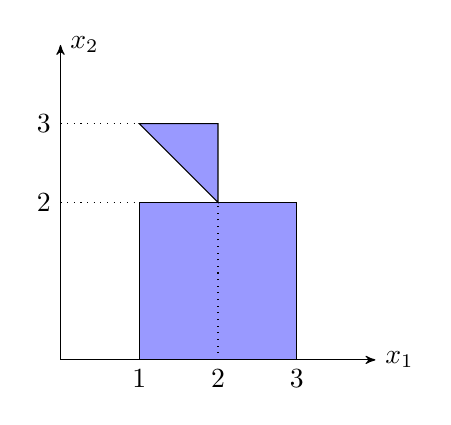
\begin{tikzpicture}
\draw[->] (0,0) -- (4,0);
\draw[->] (0,0) -- (0,4);
\node[right] at (4,0) {$x_1$};
\node[right] at (0,4) {$x_2$};
\draw[fill=blue!40] (1,0) rectangle (3,2);
\draw[fill=blue!40] (2,2) --(2,3) -- (1,3) -- cycle;
\node[below] at (1,0) {$1$};
\node[below] at (3,0) {$3$};
\draw[dotted,-] (2,0) -- (2,2);
\node[below] at (2,0) {$2$};
\draw[dotted,-] (0,2) -- (1,2);
\node[left] at (0,2) {$2$};
\draw[dotted,-] (0,3) -- (1,3);
\node[left] at (0,3) {$3$};

\end{tikzpicture}
\end{center}


\item What is the multi layer perceptron for the following step function,

\begin{center}
\begin{tikzpicture}
\draw[->] (-2,0) -- (5,0);
\draw[->] (0,-2) -- (0,5);
\node[right] at (5,0) {$x_1$};
\node[right] at (0,5) {$x_2$};

\draw[brown] (1,0) rectangle (2,3);
\draw[brown] (2,-1) rectangle (3,0);

\node[below] at (1,0) {$1$};
\node[below] at (2,0) {$2$};
\node[below] at (3,0) {$3$};

\draw[dotted,-] (0,3) -- (1,3);
\draw[dotted,-] (0,-1) -- (3,-1);

\node[left] at (0,3) {$3$};
\node[left] at (0,-1) {$-1$};

\end{tikzpicture}
\end{center}

\item Write a multi-layer perceptron to model the function $f(x)=x(2-x)$ in the interval $[0,2]$ with the step size $h=0.5$.

\begin{center}
\begin{tikzpicture}
\draw[->] (0,0) -- (4,0);
\draw[->] (0,0) -- (0,4);
\node[right] at (4,0) {$x_1$};
\node[right] at (0,4) {$x_2$};
\draw[scale=1.8, domain=0:2, smooth, variable=\x, blue,-] plot ({\x}, {\x*(2-\x)});
\node[below] at (3.6,0) {$2$};
\end{tikzpicture}
\end{center}

Help: 

\begin{center}
\begin{tikzpicture}
\draw[->] (0,0) -- (5,0);
\draw[->] (0,0) -- (0,5);
\node[right] at (5,0) {$x_1$};
\node[right] at (0,5) {$x_2$};
\draw[scale=2, domain=0:2, smooth, variable=\x, blue,-] plot ({\x}, {\x*(2-\x)});
\node[below] at (4,0) {$2$};
\draw[red] (0,0) rectangle (1,1.5);
\draw[red] (1,0) rectangle (2,2);
\draw[red] (2,0) rectangle (3,2);
\draw[red] (3,0) rectangle (4,1.5);
\node[below] at (1,0) {$0.5$};
\node[below] at (2,0) {$1$};
\node[below] at (3,0) {$1.5$};
\node[below] at (4,0) {};
\end{tikzpicture}
\end{center}



\end{enumerate}

\end{document}
